\chapter{Теоријски преглед}
\label{sec:2}

\section{Неуронске мреже}
\label{sec:4}

\subsection{Неурон}
\label{sec:4}

У контексту неуронских мрежа, неурон представља основну јединицу обраде информација \cite{noauthor_artificial_20233}. 
Он симулира рад људског неурона у мозгу. Графички изглед једног неурона је приказан на слици \ref{fig:neuron}. 
Сваки неурон прима улазне сигнале $x_0, x_1 ... x_N$, обрађује их, и издаје излазни сигнал $y$.

Тежине (енг. \textit{weights}) $w_0, w_1 ... w_N$ представљају параметре који се користе за модификацију улазних података прослеђених неурону. 
Сваки улаз у неурон је помножен са одговарајућом тежином. Тежине утичу на значајност улазних података и одређују њихову улогу у формирању излаза неурона. 
Процес учења у неуронским мрежама, познат као обука, састоји се из ажурирања и промене тежина како би мрежа најбоље моделовала жељени задатак.

Збир улаза помножених са тежинама сигнала се прослеђује активационој функцији $f$. 
Коришћењем активационих функција, неуронске мреже су у могућности да моделирају нетривијалне односе између улазних и излазних података. 
Овај излазни сигнал затим служи као улаз за следећи слој неурона у мрежи.

Пристрасност (енг. \textit{bias}) је додатни параметар који се користи за прилагођавање излаза неурона. 
Тежина којом пристрасност утиче на активациону функцију је одређена тежином $b$.

\begin{figure}[h]
    \centering
    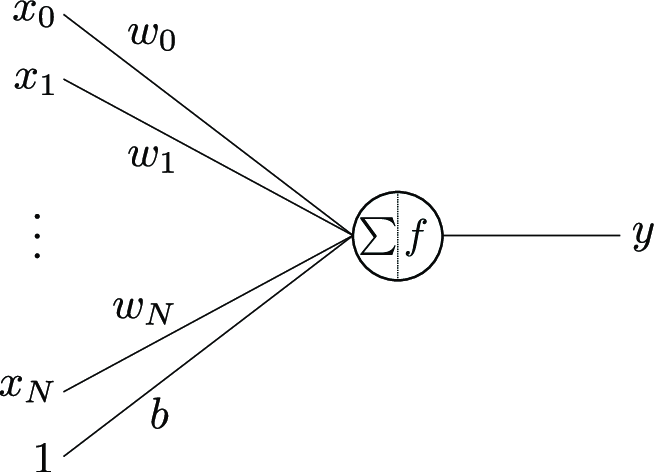
\includegraphics[width=0.7\textwidth]{images/neuron.png}
    \caption{Графички приказ једног неурона \cite{ioannou_structural_2017}}
    \label{fig:neuron}
\end{figure}

Математички израз како тежине, улази и пристрасност утичу на излазни сигнал је дат једначином \ref{eq:neuron}.

\begin{equation}
    y = f\left(\sum_{i=1}^{n} w_i x_i + b\right)
    \label{eq:neuron}
\end{equation}

\subsection{Потпуно повезане неуронске мреже}
\label{sec:41}

Потпуно повезане неуронске мреже (ППНМ) (енг. \textit{Fully Connected Neural Networks}) су скуп повезаних неурона описаних у \ref{sec:4}. 
Састоји се од више слојева, први слој се назива улазни слој, а последњи слој се назива излазни слој. 
Сви остали слојеви се називају скривени слојеви (енг. \textit{hidden layer}). 
На слици \ref{fig:fc} је графички приказана неуронска мрежа која има 2 скривена слоја.
Сваки слој може да има произвољан број неурона, а неуронска мрежа може да има произвољан број скривених слојева. 
Мењајући архитектуру, односно број неурона у једном слоју и број слојева се мења моћ мреже и комплексност задатка који мрежа може да решава.

\begin{figure}[h]
    \centering
    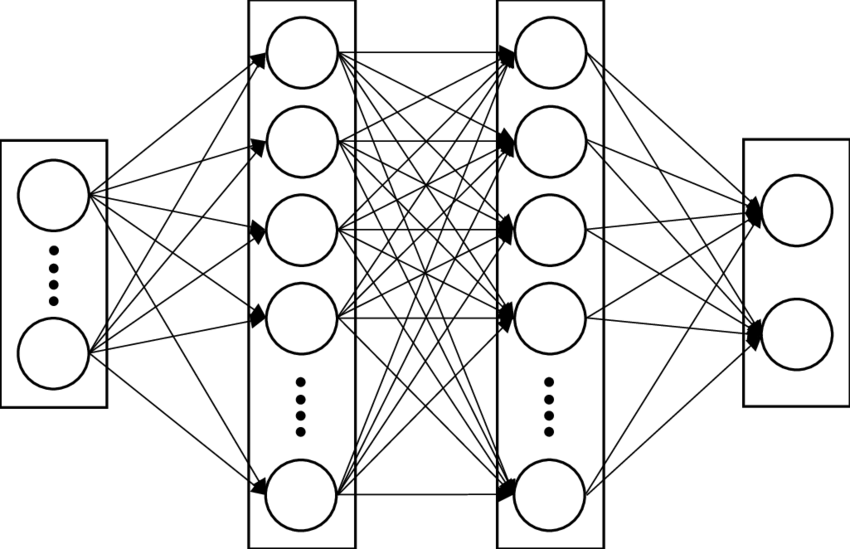
\includegraphics[width=0.7\textwidth]{images/fc.png}
    \caption{Графички приказ потпуно повезане неуронске мреже \cite{anwar_learned_2017}}
    \label{fig:fc}
\end{figure}

ППНМ прима само децималне бројеве као улаз и битно је да приликом тренирања и предикције да исте вредности атрибута улазних података улазе у потпуно повезану мрежу на исти улаз.
Овакав тип мреже се најбоље показао на проблемима класификације \cite{noauthor_artificial_2023}.

\subsection{Софтмакс (\textit{softmax})}

Софтмакс функција се често користи у неуралним мрежама за решавање задатака класификације, као и за генерисање расподеле вероватноћа излаза из мреже. 
Она трансформише илаз тако да све вредности излаза леже у интервалу између 0 и 1 и да се сума свих вредности излаза једнака 1 
Формално, софтмакс функција је дефинисана у изразу \ref{eq:ss} за вектор излаза Z :

\begin{equation}
    \label{eq:ss}
    \text{softmax}(z)_i = \frac{e^{z_i}}{\sum_{j=1}^{N} e^{z_j}}
\end{equation}

Где:

\begin{itemize}
    \item z је вектор излаза модела за сваку од N класа.
    \item e представља експоненцијалну функцију (елемент по елемент).
    \item i је индекс класе за коју рачунамо вероватноћу.
\end{itemize}

\section{Архитектура трансформера}
\label{sec:transformer}

\subsection{Токенизација}

Трансформери раде над дискретним секвенцама токена уместо над сировим текстом, па је први корак токенизација -- разлагање текста на атомске јединице (токене) које чине улаз модела. Савремени модели трансформера често користе токенизацију на нивоу подсегмената (eng. \textit{subword}) како би постигли отворени речник, што значи да се свака реч може представити као секвенца подсекмената токена. Распрострањен \textit{subword} метод је Кодирање парова бајтова (енг. Byte Pair Encoding - BPE), алгоритам за компресију података прилагођен раду са текстом. Првобитно га је представио Gage (1994) за компресију, а касније су га на сегментацију речи применили Sennrich и сар. (2016) \cite{gage_new_1994,sennrich_neural_2016}. Алгоритам итеративно спаја најфреквентнији пар симбола у корпусу, додајући тако насталу целину као нови токен. Понављањем спајања, BPE гради речник уобичајених подсегмената; на пример, ретка реч „nationalism" може се поделити на подсегменте „nation@@" и „alism" (са „@@" као ознака за поделу) на основу фреквенције. Овај процес даје речник фиксне величине састављен од подсегмената које постижу баланс између грануларности на нивоу карактера и холизма на нивоу речи. Теоријска улога токенизације је да ограничи улазни простор на управљив скуп симбола, а да притом сачува могућност да се од тих симбола конструише било која реч.

\subsection{Векторска репрезентација токена}

После токенизације, сваки токен се трансформише у континуалну векторску репрезентацију (енг. \textit{Embedding}). Теоријска улога векторске репрезентације је да омогући моделу да у наученом векторском простору мери семантичке и синтаксичке сличности између токена. Формално, овај слој се може посматрати као табела претраге -- нпр. матрица $\mathbf{E} \in \mathbb{R}^{|V| \times d}$, где је $|V|$ величина речника, а $d$ димензија скривеног слоја модела. Сваки токен $t_i$ мапира се на $d$-димензионални вектор $\mathbf{x}_i = \mathbf{E}[t_i]$. Ови вектори су параметри који се добијају обучавањем модела, иницијално насумични или претходно тренирани, и оптимизују се током обуке модела да би кодирали корисне лингвистичке информације. Код трансформера, вектори су обично величине $d_{\text{model}}$ и скалирају се са $\sqrt{d_{\text{model}}}$ при иницијализацији како би им се величина задржала у разумним границама \cite{vaswani_attention_2017}.

Важно обележје корака векторске репрезентације је додавање позиционог кодирања. За разлику од рекурентних мрежа, трансформер нема урођено поимање редоследа речи, па се позиционе информације морају експлицитно увести. Решење које предлажу Vaswani и сар. је да се сваком позиционом векторском репрезентацијом токена дода позициони вектор \cite{vaswani_attention_2017}. Ова позициона кодирања су фиксна и дефинисана су помоћу синусоидалних функција различитих фреквенција \cite{vaswani_attention_2017}. Конкретно, за позицију $pos$ (нумерисану од 0) и индекс димензије $i$, кодирање је:

\begin{equation}
\text{PE}(pos,\,2i) = \sin\!\Big(\frac{pos}{10000^{2i/d_{\text{model}}}}\Big), \qquad \text{PE}(pos,\,2i+1) = \cos\!\Big(\frac{pos}{10000^{2i/d_{\text{model}}}}\Big)
\label{eq:positional_encoding}
\end{equation}

где је $d_{\text{model}}$ димензионалност ембединга \cite{vaswani_attention_2017}. Ова наизменична синус-косинус формулација производи позиционе векторе јединствене за сваку позицију и који кодирају релативна растојања. Позиционо кодирање $\mathbf{p}_i$ се додаје вектору токена $\mathbf{x}_i$ како би се добила коначна улазна репрезентација $\mathbf{z}_i = \mathbf{x}_i + \mathbf{p}_i$ која се уводи у трансформер. Због тога модел може да разликује позиције токена и учи односе који зависе од редоследа, а да и даље ради над континуалним векторским репрезентацијама.

\subsection{Механизам пажње}

Према научном раду \cite{vaswani_attention_2017}, функција пажње (енг. \textit{Attention head}) се може описати као пресликавање упита и скупа парова кључа и вредности у излазни вектор, при чему су упит, кључеви, вредности и излаз сви вектори. Излаз се израчунава као тежинска сума вектора вредности, а тежина сваке вредности добија се из функције компатибилности између упита и одговарајућег кључа.

\subsection{Скалирана пажња заснована на скаларном производу}

Скалирана пажња заснована на скаларном производу (енг. \textit{Scaled Dot-Product Attention}) је механизам који омогућава моделу да одмери утицај различитих токена при израчунавању репрезентација за следећи слој. У трансформеру, основна јединица је глава пажње са скалираним скаларним производом. Теоријска улога једне главе пажње је да израчуна тежинску комбинацију вектора вредности за сваку позицију, где су тежине одређене паровним сличностима између упита и скупа кључева. Свака глава пажње ради над три скупа вектора: упити ($Q$), кључеви ($K$) и вредности ($V$), димензија $d_k$, $d_k$ и $d_v$ (често $d_v = d_k$) редом. У интроспективној пажњи (енг. \textit{self-attention}), језгру трансформер слојева, упити, кључеви и вредности долазе из исте секвенце, што омогућава моделу да обрађујући дату позицију „обрати пажњу" на друге позиције у секвенци. Механизам пажње израчунава меру компатибилности између сваког упита и сваког кључа помоћу скаларног производа $Q \cdot K^T$ \cite{vaswani_attention_2017}. Резултат се затим скалира са $\frac{1}{\sqrt{d_k}}$ и нормализују \textit{softmax}-ом како би се добиле тежине пажње. Излаз главе пажње је тежинска сума вектора вредности, користећи те нормализоване тежине. Математички, за скуп $Q$, $K$ и $V$, глава пажње даје:

\begin{equation}
\text{Attention}(Q, K, V) = \text{softmax}\!\Big( \frac{Q\,K^T}{\sqrt{d_k}}\Big)\,V
\label{eq:attention}
\end{equation}

како су увели Vaswani и сар. \cite{vaswani_attention_2017}. Сваки ред матрице $\text{softmax}(\frac{QK^T}{\sqrt{d_k}})$ представља расподелу вероватноће над свим кључевима за одређени упит, показујући колико пажње (значаја) упит поклања вредности сваког кључа. Добијена тежинска сума даје контекстни вектор за сваки упит, тј. излаз пажње који кодира информације агрегиране из свих позиција, пристрасно у корист оних релевантних за позицију упита.

Скалирање са $\frac{1}{\sqrt{d_k}}$ је кључан теоријски детаљ. Без њега, скаларни производи $QK^T$ расту по величини са већим $d_k$, што може да доведе тога да \textit{softmax} обрати пажњу на само један токен игноришићи остале. Скалирањем скаларних производа инверзним квадратним кореном димензије кључа, вредности које улазе у \textit{softmax} остају умерене чак и кад $d_k$ расте, што емпиријски води стабилнијем учењу \cite{vaswani_attention_2017,bahdanau_neural_2015}. У пракси, употреба скалиране пажње са скаларним производом у трансформеру обезбедила је једноставнију и бржу имплементацију пажње без жртвовања перформанси \cite{vaswani_attention_2017}. Свака глава пажње стога излази секвенцу вектора (по један по улазној позицији) који мешају информације са свих позиција, фокусирајући се на оне процењене као релевантне датом упиту.

Архитектура механизма пажње је приказама на слици \ref{fig:dot_attention}.

\begin{figure}[h]
    \centering
    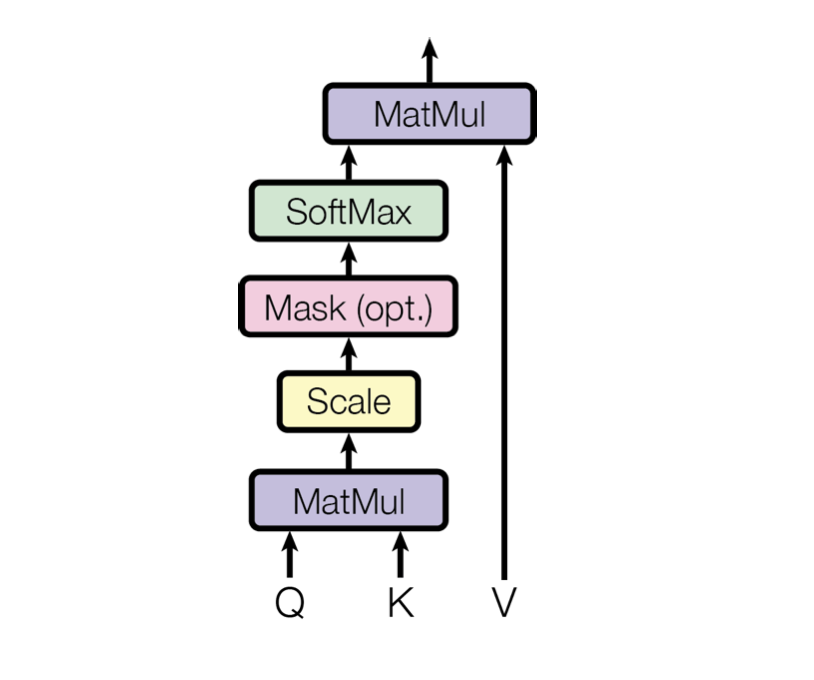
\includegraphics[width=0.7\textwidth]{images/dot-attention.png}
    \caption{Архитектура скалиране пажње засноване на скаларном производу}
    \label{fig:dot_attention}
\end{figure}

\subsection{Механизам пажње са више глава}

Иако једна глава пажње може да извуче један скуп односа преко секвенце, трансформер користи механизам пажње са више глава (енг. \textit{Multi-Head Attention}) како би моделу омогућио да паралелно обраћа пажњу на више аспеката података. Идеја је да постоји више независних глава пажње (рецимо $h$ глава), свака са сопственим линеарним трансформацијама за упите, кључеве и вредности. Улаз у слој вишеглаве пажње се прво пројектује у $h$ различитих подпростора помоћу $h$ научених линеарних пројекција: за сваку главу $i$ имамо матрице пројекција $W_i^Q$, $W_i^K$, $W_i^V$ које мапирају оригиналне $d_{\text{model}}$-димензионалне упите, кључеве и вредности у $d_k$-димензионе $Q_i$, $K_i$, $V_i$. Типично се бира $d_k = d_{\text{model}}/h$ тако да је укупна рачунања преко $h$ глава упоредива са једном „великом" главом по димензионалности. Свака глава $i$ затим изводи скалирану пажњу са скаларним производом у свом пројектованом подпростору, дајући излазну матрицу $\text{head}_i = \text{Attention}(Q_i, K_i, V_i)$ димензије $n \times d_v$ (за $n$ улазних позиција). Излази $h$ глава се конкатенирају (дуж димензије карактеристика), па се кроз завршну линеарну пројекцију $W^O$ (облика $h\cdot d_v$ на $d_{\text{model}}$) поново комбинују информације. У формулном облику, ако $i$-ти излаз главе означимо као $\text{head}_i$, излаз вишеглаве пажње је:

\begin{equation}
\text{MultiHead}(Q, K, V) = \text{Concat}(\text{head}_1, \text{head}_2, \dots, \text{head}_h)\,W^O
\label{eq:multihead}
\end{equation}

где је $\text{head}_i = \text{Attention}(Q W_i^Q, K W_i^K, V W_i^V)$ за $i=1,\dots,h$ \cite{vaswani_attention_2017}. Ова архитектура (слика \ref{fig:multi_head_attention}) ефективно покреће $h$ одвојених слојева пажње у паралели \cite{vaswani_attention_2017}. Теоријска предност вишеглаве пажње је у томе што свака глава може да учи да се фокусира на различите обрасце или односе у подацима.

\begin{figure}[h]
    \centering
    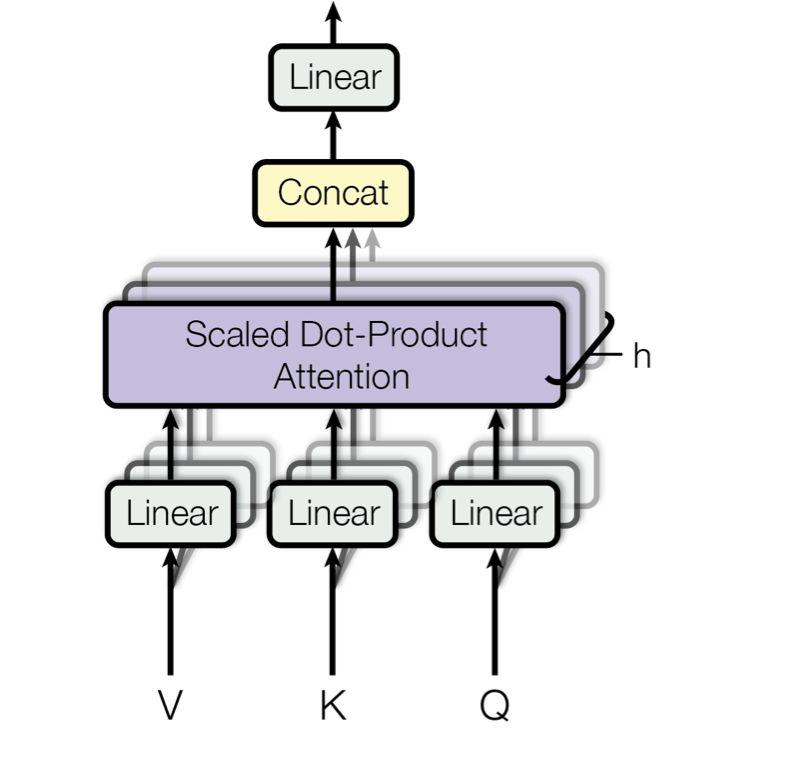
\includegraphics[width=0.7\textwidth]{images/multi-head-attention.png}
    \caption{Архитектура механизма пажње са више глава}
    \label{fig:multi_head_attention}
\end{figure}

\subsection{Трансформер}

У пуном енкодер--декодер Трансформеру (енг. \textit{Transformer}), изворна секвенца се најпре токенизује, ембедује и проширује позиционим кодирањем, након чега пролази кроз стек енкодера од N идентичних слојева. Сваки слој енкодера примењује:

\begin{enumerate}
\item механизам интроспективне пажње (\textit{self-attention}) која омогућава свакој позицији да обраћа пажњу на све остале у извору
\item позиционо-локални, по елементима, потпуно повезан (\textit{feed-forward}) слој
\end{enumerate}

оба подслеја су обавијена резидуалним („Add") везама и нормализацијом слоја („Norm"). Активности вршног слоја енкодера H представљају контекстом богате репрезентације које делују као меморија са адресирањем по садржају за декодер. Декодер конзумира на десно померену циљну секвенцу са сопственом векторском репрезентацијом и позиционим кодирањем. Сваки слој декодера садржи:

\begin{enumerate}
\item маскирану самопажњу, са каузалном (троугластом) маском тако да позиција $t$ не може да види токене $> t$
\item енкодер--декодер \textit{cross-attention}, где упити декодера претражују меморију енкодера N (кључеве/вредности), омогућавајући ослањање на извор
\item \textit{feed-forward} мрежу
\end{enumerate}

и овде резидуалне путање и нормализација слоја стабилизују оптимизацију и очувавају сигнал. Слагање слојева даје хијерархијску композицију: нижи слојеви хватају локалне синтаксичке сигнале, док виши кодирају семантичке односе, при чему механизам пажње са више глава расподељује ове улоге по главама. Коначна стања декодера пролазе кроз линеарну пројекцију и \textit{softmax} (енг. \textit{softmax}) ради добијања вероватноћа наредног токена.

Графички приказ архитектуре трансформера је приказана на слици \ref{fig:transformer}.

\begin{figure}[h]
    \centering
    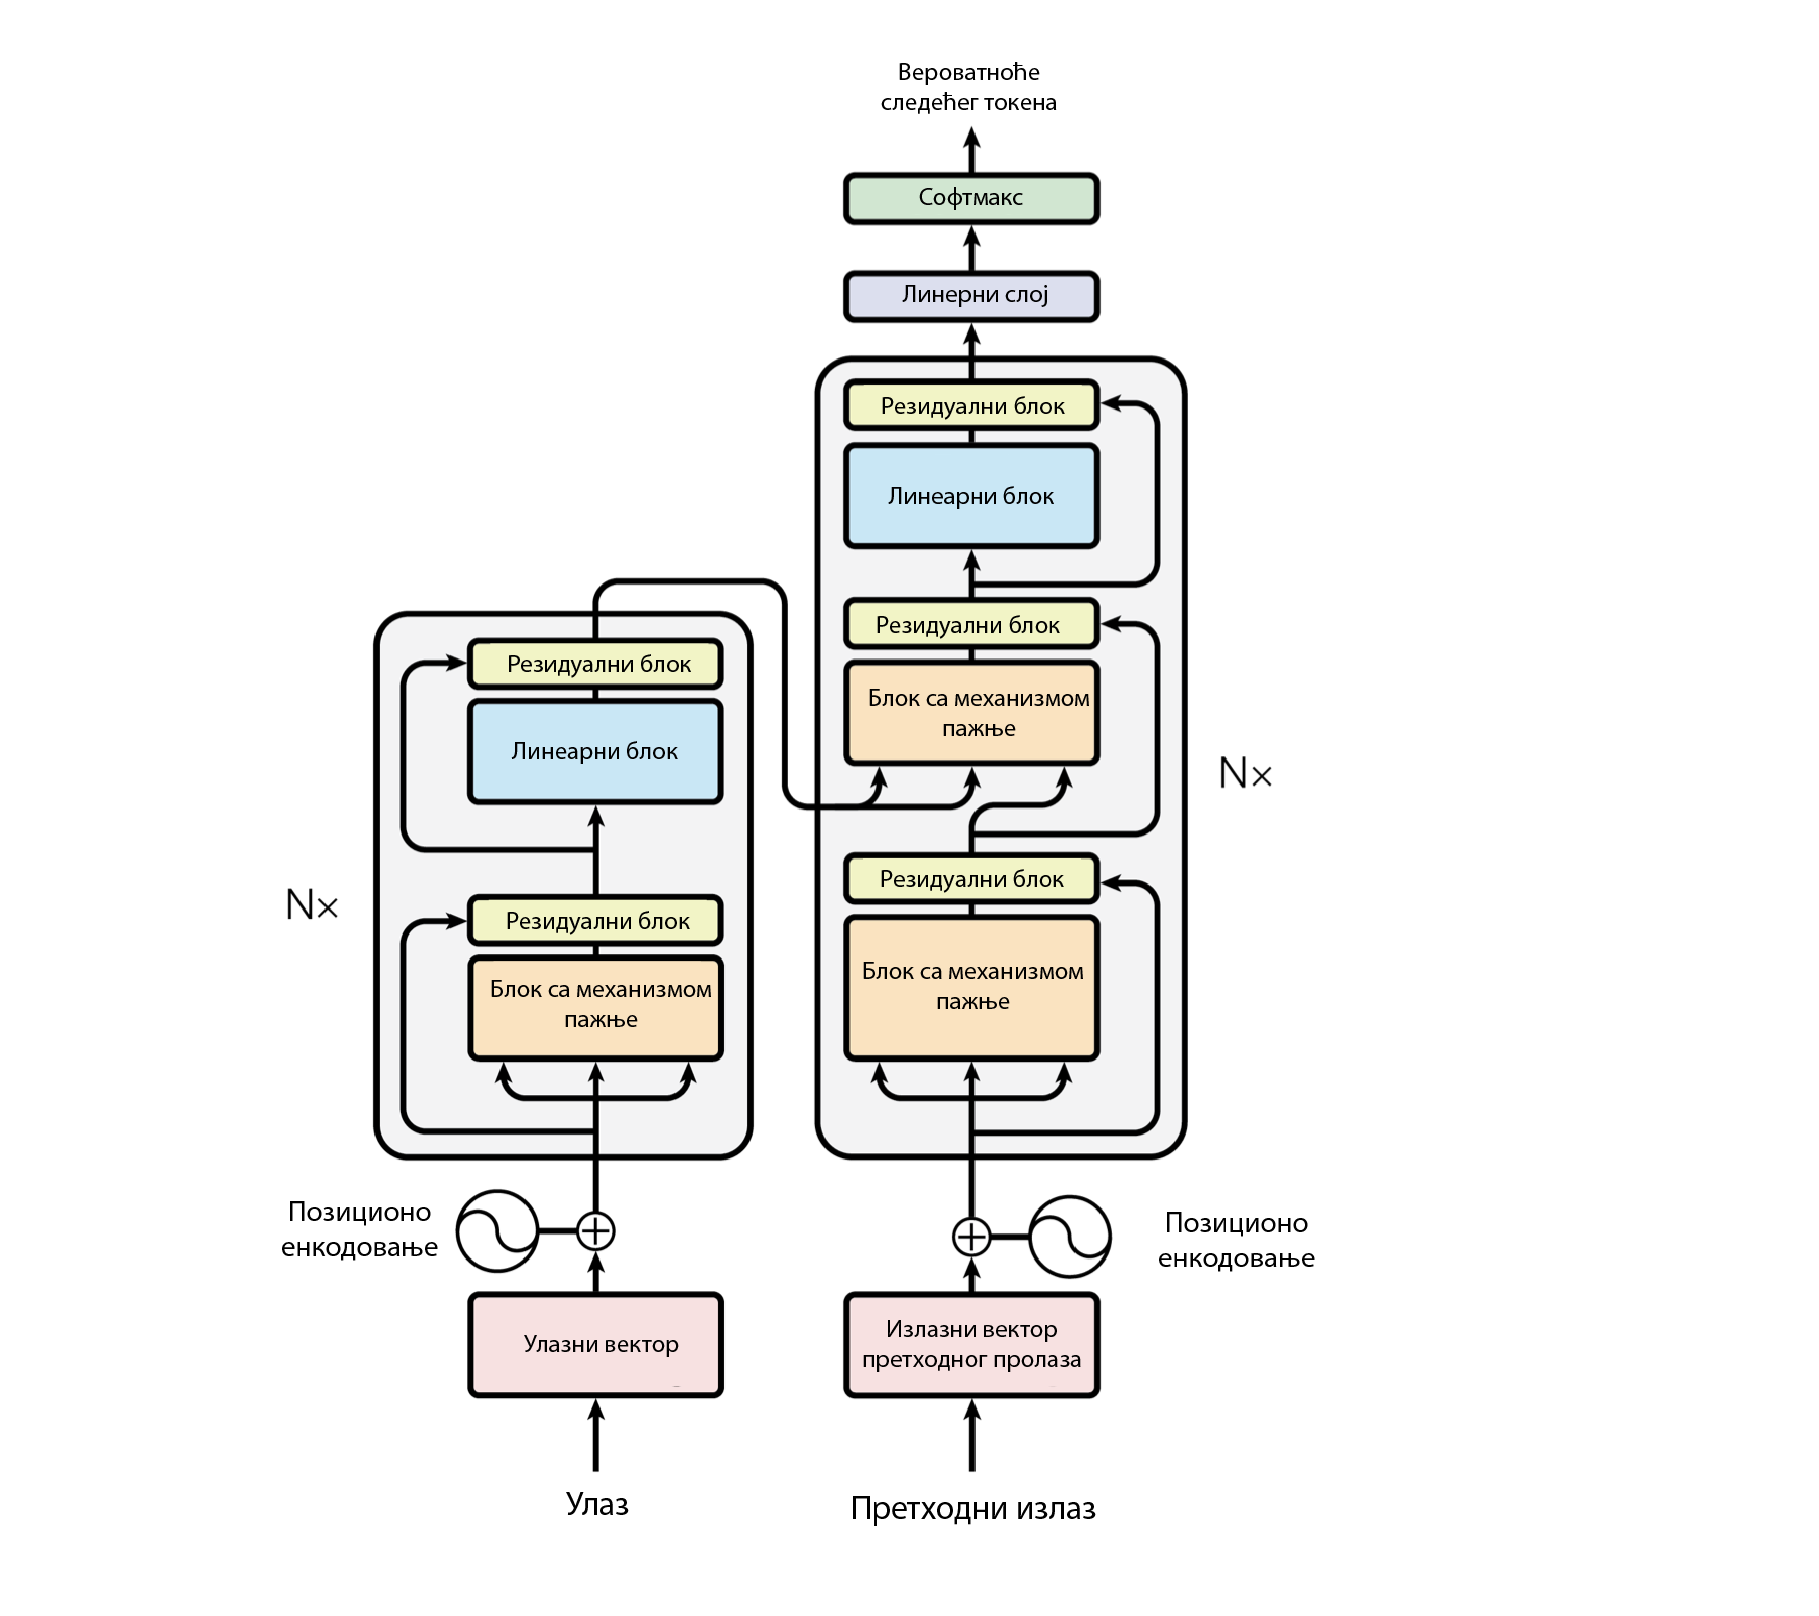
\includegraphics[width=0.9\textwidth]{images/transformer.png}
    \caption{Архитектура трансформера}
    \label{fig:transformer}
\end{figure}

\section{Архитектура великог језичког модела}
\label{sec:llm_architecture}

Велики језички модели (ВЈМ) (енг. \textit{Large Language Models - LLM}) заснивају се на трансформер архитектури \cite{vaswani_attention_2017}. ВЈМ је веома дубока хрпа трансформер слојева, при чему сваки слој садржи вишеглаву пажњу и \textit{feed-forward} подслојеве. Ова архитектура омогућава моделу да одмерава релевантност сваке речи (токена) у улазу у односу на све друге речи, хватајући далекосежне зависности у тексту. Пошто трансформер обрађује речи паралелно, може да се скалира на веома велике величине модела и ефикасно рукује дугим секвенцама \cite{vaswani_attention_2017}.

\subsection{Врсте великих језичких модела}

Иако основни трансформер блок остаје језгро, ВЈМ-ови типично имају огроман број параметара распоређених преко многих слојева. На пример, модел GPT-3 компаније OpenAI садржи 175 милијарди параметара и користи 96 трансформер слојева у конфигурацији само-декодера \cite{brown_language_2020}. Сваки слој у GPT-3 има бројне главе пажње (96 глава по слоју) које раде паралелно, што омогућава моделу да прати различите аспекте улазног текста \cite{brown_language_2020}.

Упркос својој величини, архитектура већине ВЈМ-а може се категоризовати у неколико основних типова:

\begin{itemize}
\item \textbf{само-декодерски модели} (попут серије GPT и Meta-иног LLaMA) који генеришу текст предвиђајући следећи токен
\item \textbf{само-енкодерски модели} (попут BERT-а) намењени задацима разумевања и анализе
\item \textbf{енкодер--декодер модели} (попут T5) погодни за секвенца-у-секвенцу задатке (превођење, сажимање итд.) \cite{vaswani_attention_2017,lu_large_2024}
\end{itemize}

Општенаменски ВЈМ који се користе у чет-ботовима и креативном генерисању текста обично су трансформери само-декодерског типа, претходно тренирани да настављају текст. У свим случајевима, међутим, оквир самопажње трансформера је кичма која омогућава овим моделима да из података науче сложене језичке обрасце и семантику \cite{vaswani_attention_2017}. Резултат је архитектура која, када се скалира, може да испољи изненађујуће богате способности разумевања и генерисања језика.

\subsection{Ограничења великих језичких модела}

Однос између дужине контекста и механизма пажње трансформера је директан. Механизам интроспективне пажње омогућава сваком токену да обрати пажњу на све друге токене у улазу, што је начин на који модел интегрише контекст. Али то има цену: пажња има квадратну сложеност у односу на дужину секвенце. Другим речима, удвостручавање прозора контекста може да учетворостручи потребно рачунање за пажњу \cite{vaswani_attention_2017,lu_large_2024}. Зато је дужина контекста дуго имала практична ограничења -- обрада веома дугих секвенци је спора и захтева много меморије. Тренутни ВЈМ-и се претежно тренирају на релативно кратким исечцима текста (нпр. неколико хиљада токена), што такође значи да можда природно не уче зависности у веома дугим текстовима \cite{lu_large_2024}.

%\chapter{Литература}
%\label{sec:7}

% Predlažem upotrebu bibtex i kreiranje .bib fajlova, a da se podaci za njh skidaju sa Google Scholar i sličnih servisa
\section{Контекст у великим језичким моделима}
\label{sec:llm_context}

У ВЈМ-а, контекст се односи на улазни текст који се моделу пружа и на који се модел условљава да би генерисао одговор. То чини ефективну радну меморију модела, ограничену прозором контекста одређене дужине мерене у токенима, што ограничава колико текста модел може одједном да разматра \cite{martineau_whats_2024}. Све инструкције задатка, позадинске информације и историја конверзације морају бити кодиране у овом контексту, јер LLM-ови током инференције не уче активно нове информације – уместо тога, генеришу излазе искључиво на основу образаца у датом упиту и својих тренираних параметара \cite{martineau_whats_2024}. Другим речима, све што модел треба да зна или да уради за дати упит мора бити обезбеђено у улазном контексту у тренутку извршавања. Већи прозор контекста зато омогућава да се укључи више информација или дужи дијалог, помажући моделу да током дугих интеракција производи кохерентне и релевантне одговоре \cite{martineau_whats_2024}. Међутим, преоптерећивање контекста има мане: повећава рачунање и трошак, а модели могу тешко да уоче релевантне детаље ако је промпт предугачак или има велики шум \cite{liu_lost_2023}. Истраживања показују да ВЈМ-и често испољавају пристрасности првенства и свежине – теже да се фокусирају на информације на почетку или крају прозора контекста више него на оне у средини \cite{liu_lost_2023}. Ово сугерише да редослед и позиционирање садржаја у промпту могу утицати на перформансе модела, што је важна напомена при изради ефективних упита \cite{liu_lost_2023}.

\subsection{Манипулисање контекстом путем изградње упита}

Пошто је понашање ВЈМ-а у потпуности вођено улазним текстом, могуће је манипулисање контекстом како би се модел усмерио ка различитим задацима и одговорима. Ова пракса је позната као промпт инжењеринг (енг. \textit{Prompt engineering}): формулисање правих инструкција или примера у промпту да би се изазвао жељени излаз модела. Уместо ажурирања параметара модела, промпт инжењеринг „програмира" модел природним језиком. Промптови могу бити једноставни – инструкција или питање – или сложени, са структурираним уносом који садржи више примера и ограничења. На пример, може се испред текста додати инструкција као што је „Преведи следећи текст на француски:" или „Сажми кључне тачке из овог чланка." да би се задатак усмерио \cite{sahoo_systematic_2025}. Ова способност извођења задатака по примеру у контексту, без додатног тренирања модела, обележје је модерних ВЈМ-а и често се назива учење у контексту (енг. \textit{in-context learning}) \cite{sahoo_systematic_2025}.

\paragraph{Технике манипулисања контекстом укључују:}

\begin{itemize}
  \item \textbf{Zero-Shot промптовање:} Пружање само инструкције или питања, ослањајући се на стечено знање модела за одговор (нпр. „Објасни зашто је небо плаво.") \cite{sahoo_systematic_2025}.
  \item \textbf{Few-Shot промптовање:} Давање неколико примера питање--одговор или демонстрација пре стварног упита, да би се моделу показало како да одговара. Ово помаже да се активирају релевантни обрасци из предтренинга путем примера \cite{sahoo_systematic_2025}.
  \item \textbf{Chain-of-Thought промптовање:} Инструкција моделу да резонује кроз проблем корак--по--корак (често додавањем „Хајде да размишљамо корак по корак") ради побољшања тачности у сложеном резоновању \cite{sahoo_systematic_2025}.
  \item \textbf{Промптовање улогом:} Додавање контекста који уоквирује ко је модел или стил одговора (нпр.: „Ти си стручни медицински асистент. Одговори на питање уз клиничке доказе.") \cite{sahoo_systematic_2025}.
\end{itemize}

Стратешким обликовањем контекста овим методама, из истог модела могу се откључати широки опсези способности – од писања кода до одговарања на финансијска питања – без промене самог модела \cite{sahoo_systematic_2025}.

\subsection{Генерисање са допунским преузимањем}

Иако се промпт дизајном може боље искористити оно што ВЈМ већ зна, постоје ситуације када су потребне информације које модел не зна. Генерисање са допунским преузимањем (енг. \textit{Retrieval--Augmented Generation} -- RAG) је техника која ово ограничење превазилази увођењем спољног извора знања у контекст који се даје моделу \cite{lewis_retrieval_2020}. У овом приступу, систем најпре шаље упит ка бази знања или корпусу докумената да дохвати релевантне пасусе, а затим проширује промпт тим преузетим пасусима као додатним контекстом \cite{lewis_retrieval_2020}. LLM се затим условљава овим обогаћеним контекстом да би генерисао одговор \cite{lewis_retrieval_2020}. То ефективно опрема модел динамичком, непараметарском меморијом: уместо да се ослања само на оно што је у његовим фиксним параметрима, модел може да користи ажурне информације довучене у тренутку упита \cite{lewis_retrieval_2020}.

Оваквим проширивањем контекста може значајно да се побољша учинак на задацима који захтевају знање. На пример, показано је да је RAG модел достигао добре резултате на бенчмарцима за отворене и доменске задатке са структуром питање--одговор тако што је за сваки упит преузимао релевантне исечке са Википедије \cite{lewis_retrieval_2020,yang_dual_2025}. Поред тога, ажурирање знања модела више не захтева скупо поновно тренирање -- довољно је освежити или проширити спољну базу знања, а механизам за преузимање ће довести нове информације у контекст модела \cite{lewis_retrieval_2020}.

Важно је уочити однос између генерисања са допунским преузимањем и величине прозора контекста ВЈМ-а \cite{kim_large_2024}. Када би се, хипотетички, цела база знања или многи документи могли сместити у промпт, модел би у теорији могао директно да приступи свим тим информацијама без засебног корака преузимања \cite{kim_large_2024}. Ипак, постоје практични изазови: веома велики контексти носе велике трошкове и могу довести до превеликог шума у контексту \cite{liu_lost_2023,kim_large_2024}. Стога ова техника постаје веома релевантна, нарочито за упите који захтевају прецизно издвајање мале количине релевантног знања из огромног корпуса или за праћење најновијих информација као што је случај са финансијским извештајима.